\documentclass[12pt, leqno]{article} %% use to set typesize
\usepackage{fancyhdr}
\usepackage[sort&compress]{natbib}
\usepackage[letterpaper=true,colorlinks=true,linkcolor=black]{hyperref}

\usepackage{amsfonts}
\usepackage{amsmath}
\usepackage{amssymb}
\usepackage{color}
\usepackage{tikz}
\usepackage{pgfplots}
\usepackage{listings}
%\usepackage{courier}
%\usepackage[utf8]{inputenc}
%\usepackage[russian]{babel}

\lstset{
  numbers=left,
  basicstyle=\ttfamily\footnotesize,
  numberstyle=\tiny\color{gray},
  stepnumber=1,
  numbersep=10pt,
}

\newcommand{\iu}{\ensuremath{\mathrm{i}}}
\newcommand{\bbR}{\mathbb{R}}
\newcommand{\bbC}{\mathbb{C}}
\newcommand{\calV}{\mathcal{V}}
\newcommand{\calE}{\mathcal{E}}
\newcommand{\calG}{\mathcal{G}}
\newcommand{\calW}{\mathcal{W}}
\newcommand{\calP}{\mathcal{P}}
\newcommand{\macheps}{\epsilon_{\mathrm{mach}}}
\newcommand{\matlab}{\textsc{Matlab}}

\newcommand{\ddiag}{\operatorname{diag}}
\newcommand{\fl}{\operatorname{fl}}
\newcommand{\nnz}{\operatorname{nnz}}
\newcommand{\tr}{\operatorname{tr}}
\renewcommand{\vec}{\operatorname{vec}}

\newcommand{\vertiii}[1]{{\left\vert\kern-0.25ex\left\vert\kern-0.25ex\left\vert #1
    \right\vert\kern-0.25ex\right\vert\kern-0.25ex\right\vert}}
\newcommand{\ip}[2]{\langle #1, #2 \rangle}
\newcommand{\ipx}[2]{\left\langle #1, #2 \right\rangle}
\newcommand{\order}[1]{O( #1 )}

\newcommand{\kron}{\otimes}


\newcommand{\hdr}[1]{
  \pagestyle{fancy}
  \lhead{Bindel, Spring 2021}
  \rhead{Numerics for Data Science}
  \fancyfoot{}
  \begin{center}
    {\large{\bf #1}}
  \end{center}
  \lstset{language=matlab,columns=flexible}  
}


\begin{document}
\hdr{2021-02-09}

\section{Introduction}

The title of this course is ``Numerical Methods for Data Science.''
What does that mean?  Before we dive into the course technical
material, let's put things into context.  I will not attempt to
completely define either ``numerical methods'' or ``data science,''
but will at least give some thoughts on each.

{\em Numerical methods} are algorithms that solve problems of
continuous mathematics: finding solutions to systems of linear or
nonlinear equations, minimizing or maximizing functions, computing
approximations to functions, simulating how systems of differential
equations evolve in time, and so forth.  Numerical methods are used
everywhere, and many mathematicians and scientists focus on designing
these methods, analyzing their properties, adapting them to work well
for specific types of problems, and implementing them to run fast on
modern computers.  Scientific computing, also called Computational
Science and Engineering (CSE), is about applying numerical methods ---
as well as the algorithms and approaches of discrete mathematics ---
to solve ``real world'' problems from some application field.
Though different researchers in scientific computing focus on different
aspects, they share the interplay between the domain expertise and
modeling, mathematical analysis, and efficient computation.

I have read many descriptions of {\em data science}, and have not been
satisfied by any of them.
The fashion now is to call oneself a data
scientist and (if in a university) perhaps to start a master's program
to train students to call themselves data scientists.  There are books
and web sites and conferences devoted to data science; SIAM even has a new
journal on the Mathematics of Data Science.
But what is data science, really?
Statisticians
may claim that data science is a modern rebranding of statistics.
Computer scientists may reply that it is all about machine
learning\footnote{The statisticians could retort that machine learning
  is itself a modern rebranding of statistics, with some
  justification.} and scalable algorithms for large data sets.
Experts from various scientific fields might claim the name of data
science for work that combines statistics, novel algorithms, and new
sources of large scale data like modern telescopes or DNA sequencers.
And from my biased perspective, data science sounds a lot like scientific computing!

Though I am uncertain how data science should be defined, I am certain
that a foundation of numerical methods should be involved.  Moreover,
I am certain that advances in data science, broadly construed, will
drive research in numerical method design in new and interesting
directions.  In this course, we will explore some of the fundamental
numerical methods for optimization, numerical linear algebra, and
function approximation, and see the role they play in different styles of
data analysis problems that are currently in fashion.  In particular,
we will spend roughly two weeks each talking about
\begin{itemize}
\item Linear algebra and optimization concepts for ML.
\item Latent factor models, factorizations, and analysis of
  matrix data.
\item Low-dimensional structure in function approximation.
\item Function approximation and kernel methods.
\item Numerical methods for graph data analysis.
\item Methods for learning models of dynamics.
\end{itemize}

You will not strictly need to have a prior numerical analysis course
for this course, though it will help (the same is true of prior ML
coursework).  But you should have a good grounding in calculus and
linear algebra, as well as some ``mathematical maturity''.  I have
posted some
\href{https://www.cs.cornell.edu/courses/cs6241/2021sp/background.pdf}
to remind you of some things you may have forgotten, and perhaps to
fill in some things you may not have seen.  In addition, the readings
section of the home page consists of a number of basic (and
not-so-basic) texts to which you can refer.  Along with course notes,
we will be using chapters from some of these books (and sometimes
research papers) as required reading.  Please do ask questions as we
go, and if you see anything that you think should be corrected or
clarified, send me an email (or you can suggest a change on the course
GitHub repository.

\section{What does a matrix mean?}

\subsection{Linear algebra objects and matrix representations}

I like to think about four fundamental objects in linear algebra
involving maps on or between abstract vector spaces $\mathcal{V}$
and $\mathcal{U}$:
\begin{enumerate}
\item A {\em linear map} $\mathcal{A} : \mathcal{V} \rightarrow \mathcal{U}$
  satisfies $\mathcal{A}(v+w) = \mathcal{A}v + \mathcal{A}w$ and
  $\mathcal{A} (\alpha v) = \alpha \mathcal{A} v$ for any vectors $v,
  w \in \mathcal{V}$ and scalar $\alpha$.
\item An {\em operator} $\mathcal{A} : \mathcal{V} \rightarrow
  \mathcal{V}$ represents a mapping of a space onto itself.
\item A {\em bilinear form}
  $a : \mathcal{V} \times \mathcal{U} \rightarrow \bbR$
  is linear in both the first and the second argument.
  If $\mathcal{V}$ and $\mathcal{U}$ are vector fields over $\bbC$,
  it is natural to instead consider {\em sesquilinear forms},
  which are linear in the first argument and in the conjugate of the
  second argument.
\item A {\em quadratic form} $\phi : \mathcal{V} \rightarrow \bbR$ is
  $\phi(v) = a(v,v)$ where $a : \mathcal{V} \times \mathcal{V}
  \rightarrow \bbR$ is a
  bilinear form (real case) or sesquilinear form (complex case).  
\end{enumerate}

All four of these objects appear in various applications in
data analysis.  Linear maps between different spaces are
a basic building block for regression and function approximation;
operators are used to describe linear time invariant systems, such as
Markov chains; bilinear forms model the similarity between pairs of objects
represented by vectors $v$ and $u$; and quadratic forms are used to
measure a variety of quantities of interest in network analysis, such
as cut sizes and edge densities.

The abstract objects of linear algebra can be realized concretely
as matrices with a choice of bases.  One way of thinking of a basis
is as an invertible map from a concrete vector space (like $\bbR^n$)
to an abstract vector space (like $\mathcal{V}$).  Taking this
perspective, we write a basis for $\mathcal{V}$ as the
``quasimatrix''
\[
  V = \begin{bmatrix} v_1 & \ldots &v_n \end{bmatrix}
\]
where each column is a vector in $\mathcal{V}$, allowing us to write
an expansion of a general vector $v \in \mathcal{V}$ compactly as
\[
  v = \sum_{j=1}^n v_j x_j = Vx.
\]
We can similarly write a basis for $\mathcal{U}$ as the quasimatrix
\[
  U = \begin{bmatrix} u_1 & \ldots &u_m \end{bmatrix}.
\]
With this notation in place, we have the following matrix
representations
\begin{enumerate}
\item We represent a linear map $\mathcal{A} : \mathcal{V} \rightarrow
  \mathcal{U}$ by the matrix $A = U^{-1} \mathcal{A} V$.  Then the abstract
  operation $u = \mathcal{A} v$ is equivalent to the concrete
  matrix-vector product $y = Ax$, where $u = Uy$ and $v = Vx$.
\item We represent a bilinear form $a : \mathcal{V} \times \mathcal{U}
  \rightarrow \bbR$ as $a(Vx, Uy) = y^T A x$.
\item We represent an operator $\mathcal{A}$ by
  $A = V^{-1} \mathcal{A} V$ --- just as with a linear map between two
  spaces, but restricted to a single choice of basis.
\item We represent a quadratic form $\phi : \mathcal{V} \rightarrow \bbR$
  as $\phi(Vx) = x^T A x$ for some symmetric matrix $A$.
\end{enumerate}

\subsection{Canonical forms and decompositions}

Given a good choice of basis, we can find matrix representations with
very simple forms, sometimes called {\em canonical forms}.  For
general choices of matrices, the canonical forms are
\begin{itemize}
\item For a linear map, we have the canonical form
  \[
    A = U^{-1} \mathcal{A} V = \begin{bmatrix} I_k & 0 \\ 0 & 0 \end{bmatrix}
  \]
  where $k$ is the rank of the matrix and the zero blocks are sized
  so the dimensions make sense.
\item For an operator, we have the {\em Jordan canonical form},
  \[
    J = V^{-1} \mathcal{A} V =
    \begin{bmatrix} J_{\lambda_1} \\ & J_{\lambda_2} \\ & & \ddots
    J_{\lambda_r} \end{bmatrix}
  \]
  where each $J_{\lambda}$ is a Jordan block with $\lambda$ down the
  main diagonal and 1 on the first superdiagonal.
\item For a quadratic form, we have the canonical form
  \[
  a(Vx) = \sum_{i=1}^{k_+} x_i^2 - \sum_{i=k_++1}^{k_++k_-} x_i^2
        = x^T A x, \quad A = \begin{bmatrix} I_{k_+} \\ & -I_{k_-} \\ &
          & 0_{k_0} \end{bmatrix}.
  \]
  The integer triple $(k_+, k_0, k_-)$ is sometimes called the {\em inertia}
  of the quadratic form (or {\em Sylvester's inertia}).
\end{itemize}

As beautiful as these canonical forms are, they are terrible for
computation.  In general, they need not even be continuous!
However, if $\cal{V}$ and $\cal{U}$ have inner products, it makes
sense to restrict our attention to orthonormal bases.  This
restriction gives canonical forms that we tend to prefer in practice:
\begin{itemize}
\item For a linear map, we have the canonical form
  \[
    U^{-1} \mathcal{A} V = \begin{bmatrix} \Sigma_k & 0 \\ 0 & 0 \end{bmatrix}
  \]
  where $k$ is the rank of the matrix and the zero blocks are sized
  so the dimensions make sense.  The matrix $\Sigma_k$ is a diagonal
  matrix of {\em singular values}
  \[
    \sigma_1 \geq \sigma_2 \geq \ldots \geq \sigma_k > 0,
  \]
  and the bases $U$ and $V$ consist of the {\em singular vectors}.  
\item For an operator, we have the {\em Schur canonical form},
  \[
    V^{-1} \mathcal{A} V = T
  \]
  where $T$ is an upper triangular matrix (in the complex case) or
  a quasi-upper triangular matrix that may have 2-by-2 blocks
  (in the case of a real matrix with complex eigenvalues).
  In this case, the basis vectors span nested invariant subspaces
  of $\mathcal{A}$.
\item For a quadratic form, we have the canonical form
  \[
    a(Vx) = \sum_{i=1}^{n} \lambda_i x_i^2 = x^T \Lambda x,
  \]
  where $\Lambda$ is a diagonal matrix with $\lambda_1, \ldots,
  \lambda_n$ on the diagonal.
\end{itemize}

If we compute canonical forms for matrices (rather than for abstract
operators), we have some of the standard matrix decompositions that
appear in numerical linear algebra:
\begin{itemize}
\item The Singular Value Decomposition (SVD):
  \[
    A = U \Sigma V^*
  \]
\item The Jordan decomposition (square $A$):
  \[
    A = V J V^{-1}
  \]
\item The Schur decomposition (square $A$):
  \[
    A = V T V^{*}
  \]
\item The symmetric eigendecomposition (symmetric $A$)
  \[
    A = V \Lambda V^*
  \]
\end{itemize}
When $A$ is symmetric, the latter three decompositions are the same.
When $A$ is in addition positive semi-definite, all four decompositions
coincide.  In general, though, the ``right'' canonical decomposition
depends on the type of linear algebraic object we are working with.

\section{Optimization}

Much of this class\footnote{%
  There are also some topics in the class that do not fit naturally
  into an optimization framework, and we will deal with them as they come.
} will involve different types of optimization problems:
\begin{equation}
  \mbox{minimize } \phi(x) \mbox{ s.t. } x \in \Omega.
\end{equation}
Here $\phi : \bbR^n \rightarrow \bbR$ is the {\em objective function} and 
$\Omega$ is the {\em constraint set}, usually defined in terms of a
collection of constraint equations and inequalities:
\[
\Omega = \{ x \in \bbR^n :
  c_i(x) = 0, i \in \mathcal{E} \mbox{ and }
  c_i(x) \leq 0, i \in \mathcal{I} \}.
\]
A point in $\Omega$ is called {\em feasible}; points outside
$\Omega$ are {\em infeasible}.  In many cases, we will be able to
solve {\em unconstrained} problems where $\Omega$ is the entire domain of
the function (in this case, all of $\bbR^n$), so that every point is
feasible.

\begin{figure}
  \begin{center}
  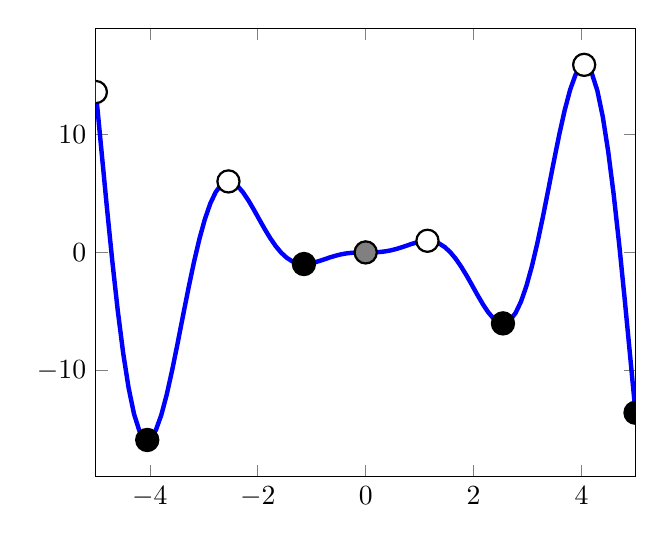
\begin{tikzpicture}
  \begin{axis}[xmin=-5,xmax=5]
    \addplot[domain=-5:5, samples=100, blue, ultra thick] (x,
            {x*x*(sin(deg(2*x)))});
    \filldraw [fill=black, thick] (axis cs:2.5435,-6.0207)
              circle [radius=4pt];
    \filldraw [fill=black, thick] (axis cs:-4.0481,-15.909)
              circle [radius=4pt];
    \filldraw [fill=black, thick] (axis cs:-1.1445,-0.98633)
              circle [radius=4pt];
    \filldraw [fill=black, thick] (axis cs:5,-13.601)
              circle [radius=4pt];
    \filldraw [fill=white, draw=black, thick] (axis cs:-2.5435,6.0207)
              circle [radius=4pt];
    \filldraw [fill=white, draw=black, thick] (axis cs:4.0481,15.909)
              circle [radius=4pt];
    \filldraw [fill=white, draw=black, thick] (axis cs:1.1445,0.98633)
              circle [radius=4pt];
    \filldraw [fill=white, draw=black, thick] (axis cs:-5,13.601)
              circle [radius=4pt];
    \filldraw [fill=black!50, draw=black, thick] (axis cs:0,0)
              circle [radius=4pt];
  \end{axis}
  \end{tikzpicture}
  \caption{The objective $\phi(x) = x^2 \sin(2x)$ on $\Omega = [-5,5]$
    has four local minima (black), along with four maxima (white) and
    one critical point which is neither (gray).  Most optimizers will
    only find one of the local minima, unless they are provided with
    a good initial guess at the global optimum.}
  \end{center}
\end{figure}

Even simple optimization problems need not have a solution.
For example, a function might not be bounded from below (e.g.~the
identity function $x \mapsto x$ on $\Omega = \bbR$), or there might
be an asymptotic lower bound that can never be achieved (e.g.~the
function $x \mapsto 1/x$ on $\Omega = \{ x \in \bbR : x > 0 \}$).
If $\phi$ is continuous and $\Omega$ is closed and bounded (i.e.~a
{\em compact} subset of $\bbR^n$), then at least there is some
$x_* \in \Omega$ that solves the global optimization problem problem:
that is, $\phi(x_*) \leq \phi(x)$ for all other $x \in \Omega$.
But just because a solution exists does not mean it is easy to
compute!  If all we know is that $\phi$ is continuous and $\Omega$ is
compact, any algorithm that provably converges to the global minimizer
must eventually sample densely in $\Omega$\footnote{%
  See {\em Global optimization} by T{\"o}rn and {\v{Z}}ilinskas.
}.  This statement of gloom
is usually too pessimistic, because we generally know more properties
than simple continuity of $\phi$.  Nonetheless, in many cases,
it may be too expensive to solve the global optimization
problem, or at least to prove that we have solved the problem.
In these cases, the best we know how to do in practices is to find a
good {\em local} minimizer, that is, a point $x_* \in \Omega$ such that
$\phi(x_*) \leq \phi(x)$ for all $x \in \Omega$ close enough to $x_*$.
If the inequality is strict, we call $x_*$ a {\em strong} local
minimizer.

The picture is rosier when we want to solve a {\em convex} problem; that is,
\begin{enumerate}
\item The {\em set} $\Omega$ is convex: $\forall x, y \in \Omega$, 
  we have $\alpha x + (1-\alpha) y \in \Omega$ for $0 < \alpha < 1$.
\item The {\em function} $\phi$ is convex on $\Omega$:
  for any $x, y \in \Omega$ and $0 < \alpha < 1$,
  \[
    \phi\left( \alpha x + (1-\alpha) y\right) \leq
    \alpha \phi(x) + (1-\alpha) \phi(y).
  \]
  If the inequality is strict, we say $\phi$ is {\em strongly} convex.
\end{enumerate}
For a convex problem, every local minimizer is also a global
minimizer, and the local minimizers (if there is more than one) form a
convex set.  If the function $\phi$ is strongly convex, then there is
only one minimizer for the problem.  Moreover, we have simple
algorithms that we can prove converge to the solution of a strongly
convex problem, though we might still decide we are unhappy about the
cost of these methods for large problems.

Whether or not they are convex, many of the optimization problems that
arise in machine learning and data science have special structure,
and we can take advantage of this structure when we develop
algorithms.  For example:
\begin{itemize}
\item
  Among the simplest and most widely used optimization problems
  are {\em linear programs}, where
  \[
    \phi(x) = c^T x
  \]
  subject to constraints $Ax \leq b$ and $x \geq 0$.  Among their many
  other uses, linear programs are a building block for
  {\em sparse recovery} methods in which we seek to represent a signal
  vector as a linear combination of a small number of elements in some
  dictionary set.  We will not discuss sparse recovery in detail, but
  will touch on it when we discuss {\em matrix completion} next week.

\item
  Unconstrained problems with {\em quadratic} objective functions
  \[
    \phi(x) = \frac{1}{2} x^T A x + b^T x + c
  \]
  are another simple and useful type.  A common special case is the
  {\em linear least squares} objective
  \[
    \phi(x) = \frac{1}{2} \|Ax-b\|^2
    = \frac{1}{2} x^T A^T A x - b^T Ax + \frac{1}{2} b^T b.
  \]
  We constantly optimize quadratic functions, both because they are
  useful on their own and because optimization of quadratics is a
  standard building block for more complicated problems.  Optimizing
  a quadratic objective is the same as solving a linear system, and
  so we can bring to bear many methods of modern linear algebra when
  solving this problem.  For example, a particularly popular approach
  is the {\em conjugate gradient} method.

\item
  In many cases, the objective is a sum of simple terms:
  \[
    \phi(x) = \sum_{i=1}^n \phi_i(x).
  \]
  An important case is the {\em nonlinear least squares} problem
  $\phi(x) = \|f(x)\|^2$, which we will discuss later this week.
  In modern machine learning, problems of this form are often solved
  by various {\em stochastic gradient} methods.
  
\item
  Most {\em spectral} methods in data science can be phrased in
  terms of the {\em quadratically constrained quadratic program}
  \[
    \phi(x) = \frac{1}{2} x^T A x + b^T x + c, \quad
    \Omega = \{ x \in \bbR^n : x^T M x = 1 \}.
  \]
  We will see such problems in matrix data analysis and also graph
  clustering and partitioning methods.  We can sometimes create methods
  for these problems that build on the fact that we have good methods
  for solving eigenvalue problems.

\item
  Some nonconvex objectives are {\em bi-convex}:
  $\phi(x_1, x_2)$ is a convex function of $x_1$ for a fixed
  $x_2$ and vice-versa, though not in $x$ as a whole.
  We will see these types of problems repeatedly
  when we consider analysis of matrix data.  We can sometimes create
  methods for these problems based on the idea of
  {\em block coordinate descent} (also known as {\em nonlinear Gauss-Seidel}
  or {\em alternating iterations}) that solve a sequence of convex
  subproblems in each of the variables in turn.

\item
  We also consider problems where
  $\phi$ (and possibly $\Omega$) depend on an additional parameter
  $s$; for example, in an optimization problem coming from regression,
  we might have an additional {\em regularization parameter}.  In this
  case, we might consider {\em continuation} methods that 
  compute the curve of solutions.
  
\end{itemize}

\end{document}
